%!TEX encoding = UTF-8 Unicode
\documentclass{beamer}


\usetheme{Madrid} % Personalización del tema 
\usecolortheme{beaver}
% Block normal
\setbeamercolor{block title}{bg=red, fg=white}
\setbeamercolor{block body}{bg=red!10, fg=black}

% Block de alerta
\setbeamercolor{block title alerted}{bg=red!80, fg=white}
\setbeamercolor{block body alerted}{bg=red!10, fg=black}

% Block de ejemplo
\setbeamercolor{block title example}{bg=red!60, fg=white}
\setbeamercolor{block body example}{bg=red!10, fg=black}

\setbeamertemplate{navigation symbols}{} % Para eliminar los símbolos clickables de navegación
\setbeamercolor{item projected}{bg=red!70!black, fg=white}
\setbeamercolor{subitem projected}{bg=red!70!black, fg=white}

\setbeamercolor{frametitle}{bg=black!80, fg=white} % Color del fondo de los títulos

% Cambia el bloque de la derecha en el pie de página (donde está la fecha/página)
\setbeamercolor{date in head/foot}{bg=black!80, fg=white}

% Si usas una barra lateral o bloques que aún se vean grises:
\setbeamercolor{structure}{fg=black!80}

\setbeamercolor{item}{fg=red!70!black}
\setbeamercolor{subitem}{fg=red!70!black}
\setbeamercolor{item projected}{bg=red!70!black, fg=white}

\setbeamertemplate{itemize item}[circle]
\setbeamertemplate{itemize subitem}[circle]

%: PAQUETES DE LATEX
%%%%%%%%%%%%%%%%%%%%%%%%%%%%%%%%%%%%
%%%%%%%%%%%%%%%%%%%%%%%%%%%%%%%%%%%%
%%%%%%%%%%%%%%%%%%%%%%%%%%%%%%%%%%%%
%%%%%%%%%%%%%%%%%%%%%%%%%%%%%%%%%%%%
%%%%%%%%%%%%%%%%%%%%%%%%%%%%%%%%%%%%
%%%%%%%%%%%%%%%%%%%%%%%%%%%%%%%%%%%%

\usepackage{tikz}


%: Paquetes básicos
\usepackage[utf8]{inputenc} % Para la codificación unicode
\usepackage[T1]{fontenc} %Para la codificación unicode
\usepackage[spanish]{babel} % Para trabajar en castellano
\usepackage{graphicx} % Para insertar imágenes
\usepackage{csquotes} % Para las citas de la bibliografía

%: Paquetes matemáticos
\usepackage{amsfonts} % Añade letras góticas, negritas... etc
\usepackage{amsmath, amssymb, amsthm} % Para alinear fórmulas y ecuaciones, añadir símbolos básicos, escribir teoremas y demos...
\usepackage{mathtools} % Para facilitar la escritura de matemáticas
\usepackage{mathrsfs} % Añade estilos para escribir símbolos
\usepackage{stmaryrd} % Añade más símbolos
\usepackage{cases} % Para distinguir casos al definir una función
\usepackage{framed} % Para recuadrar fórmulas y texto
\usepackage{tikz-cd} % Para crear diagramas con flechas
\usepackage{relsize} % Para cambiar el tamaño de fuente matemática
\usetikzlibrary{babel}
\usepackage{tikz}
\usetikzlibrary{tikzmark, arrows.meta}
\usepackage{bold-extra}




%%%%%%%%%%%%%%%%%%%%%%%%%%%%%%%%%%%%
%%%%%%%%%%%%%%%%%%%%%%%%%%%%%%%%%%%%
%%%%%%%%%%%%%%%%%%%%%%%%%%%%%%%%%%%%
%%%%%%%%%%%%%%%%%%%%%%%%%%%%%%%%%%%%
%%%%%%%%%%%%%%%%%%%%%%%%%%%%%%%%%%%%
%%%%%%%%%%%%%%%%%%%%%%%%%%%%%%%%%%%%

%: COMANDOS PERSONALIZADOS
%%%%%%%%%%%%%%%%%%%%%%%%%%%%%%%%%%%%
%%%%%%%%%%%%%%%%%%%%%%%%%%%%%%%%%%%%
%%%%%%%%%%%%%%%%%%%%%%%%%%%%%%%%%%%%
%%%%%%%%%%%%%%%%%%%%%%%%%%%%%%%%%%%%
%%%%%%%%%%%%%%%%%%%%%%%%%%%%%%%%%%%%
%%%%%%%%%%%%%%%%%%%%%%%%%%%%%%%%%%%%

%: Colores
\usepackage[dvipsnames]{xcolor}
% Comandos para resaltar con colores
\newcommand{\contrastcolor}{Blue3}
\newcommand{\headingscolor}{Blue1}
% Texto en color
\newcommand{\red}[1]{\textcolor{red}{\hspace{0pt}#1}}
\newcommand{\green}[1]{\textcolor{Green3}{\hspace{0pt}#1}}
\newcommand{\blue}[1]{\textcolor{SteelBlue3}{\hspace{0pt}#1}}
\newcommand{\garnet}[1]{\textcolor{DarkRed}{\hspace{0pt}#1}}
% En español
\let\rojo\red
\let\verde\green
\let\azul\blue
\let\granate\garnet

\def\eqref#1{\textcolor{DarkRed}{{(\ref{#1})}}} % Redefine el estilo de las referencias a ecuaciones

\usepackage{tcolorbox}

\newenvironment{teorema}[1][]{
  \begin{tcolorbox}[colback=darkred!10, colframe=darkred!90, title=Teorema\ #1, fonttitle=\bfseries]
}{
  \end{tcolorbox}
}

\newenvironment{lema}[1][]{
  \begin{tcolorbox}[colback=red!10, colframe=red!60!black, title=Lema\ #1, fonttitle=\bfseries]
}{
  \end{tcolorbox}
}

\newenvironment{definicion}[1][]{
  \begin{tcolorbox}[colback=red!10, colframe=red!80!black, title=Definición\ #1, fonttitle=\bfseries]
}{
  \end{tcolorbox}
}

\newenvironment{proposicion}[1][]{
  \begin{tcolorbox}[colback=darkred!10, colframe=darkred!70, title=Proposición\ #1, fonttitle=\bfseries]
}{
  \end{tcolorbox}
}


\let\demo\undefined
\let\enddemo\undefined
\newenvironment{demo}{%
  \par\medskip\noindent\textbf{Demostración.}\hspace{0.5em}%
}{%
  \hfill$\blacksquare$\par\medskip%
}

\let\ejmplo\undefined
\let\endejemplo\undefined
\newenvironment{ejemplo}{%
  \par\medskip\noindent\textbf{Ejemplo.}\hspace{0.5em}%
}

\newcommand{\rboxed}[1]{%
  \fcolorbox{red!80!black}{red!10}{$#1$}%
}

%%%%%%%%%%%%%%%%%%%%%%%%%%%%%%%%%%%%
%%%%%%%%%%%%%%%%%%%%%%%%%%%%%%%%%%%%
%%%%%%%%%%%%%%%%%%%%%%%%%%%%%%%%%%%%
%%%%%%%%%%%%%%%%%%%%%%%%%%%%%%%%%%%%
%%%%%%%%%%%%%%%%%%%%%%%%%%%%%%%%%%%%
%%%%%%%%%%%%%%%%%%%%%%%%%%%%%%%%%%%%


%: MACROS PERSONALIZADAS 
%%%%%%%%%%%%%%%%%%%%%%%%%%%%%%%%%%%%
%%%%%%%%%%%%%%%%%%%%%%%%%%%%%%%%%%%%
%%%%%%%%%%%%%%%%%%%%%%%%%%%%%%%%%%%%
%%%%%%%%%%%%%%%%%%%%%%%%%%%%%%%%%%%%
%%%%%%%%%%%%%%%%%%%%%%%%%%%%%%%%%%%%
%%%%%%%%%%%%%%%%%%%%%%%%%%%%%%%%%%%%

%: ABREVIATURAS BÁSICAS
%%%%%%%%%%%%%%%%%%%%%%%%%%%%%%%%%%%%
%%%%%%%%%%%%%%%%%%%%%%%%%%%%%%%%%%%%
%%%%%%%%%%%%%%%%%%%%%%%%%%%%%%%%%%%%
%%%%%%%%%%%%%%%%%%%%%%%%%%%%%%%%%%%%
%%%%%%%%%%%%%%%%%%%%%%%%%%%%%%%%%%%%

%: Conjuntos y estructuras
\newcommand{\N}{\mathbb{N}} % Naturales
\newcommand{\Z}{\mathbb{Z}} % Enteros
\newcommand{\Q}{\mathbb{Q}} % Racionales
\newcommand{\R}{\mathbb{R}} % Reales
\newcommand{\C}{\mathbb{C}} % Complejos
\renewcommand{\O}{\mathcal{O}} % Anillo de funciones o de enteros
\newcommand{\F}{\mathscr{F}} % Anillo de series formales
\newcommand{\poly}{\mathbb{P}} % Anillo de polinomios
\newcommand{\field}{\mathbb{K}} % Cuerpo genérico
\newcommand{\formal}{\field \llbracket T \rrbracket} % Anillo de series formales
\newcommand{\maximal}{\mathfrak{m}}

%: Operadores
% \ker ya viene definido
\DeclareMathOperator*{\coker}{coker} % Coker
% \dim ya viene definido
\DeclareMathOperator*{\codim}{codim} % Codimensión
\DeclareMathOperator*{\rg}{rg} % Rango
\DeclareMathOperator{\gr}{gr} % Grado
\DeclareMathOperator{\mcd}{mcd} % Máximo común divisor
\DeclareMathOperator{\mcm}{mcm} % Mínimo común múltiplo
\DeclareMathOperator{\sop}{sop} % Soporte
\DeclareMathOperator*{\Hom}{Hom} % Morfismos
\DeclareMathOperator*{\End}{End} % Endomorfismos
\DeclareMathOperator*{\Aut}{Aut} % Automorfismos
\DeclareMathOperator*{\Der}{Der} % Derivaciones
\DeclareMathOperator*{\Sh}{Sh(\mathbb{P})} % Sucesiones de Sheffer
\DeclareMathOperator*{\App}{App(\mathbb{P})} % Sucesiones de Appel
\DeclareMathOperator*{\Umb}{Umb(\mathbb{P})} % Sucesiones asociadas
\DeclareMathOperator*{\TrasUmb}{Tras_{Umb}(\mathbb{P})} % Traslaciones umbrales
\DeclareMathOperator*{\TrasSh}{Tras_{Sh}(\mathbb{P})} % Traslaciones de Sheffer
\DeclareMathOperator*{\spec}{Spec} % Espectro
\DeclareMathOperator*{\ord}{ord} % Orden
\DeclareMathOperator*{\res}{res} % Residuo
\DeclareMathOperator{\Arg}{Arg} % Argumento
\DeclareMathOperator{\Log}{Log} % Logaritmo principal
\DeclareMathOperator{\dlog}{dlog} % Derivada logarítmica
\renewcommand\Re{\operatorname{Re}} % Parte real
\renewcommand\Im{\operatorname{Im}} % Parte imaginaria

%: Lógica
\newcommand{\ssi}{\Leftrightarrow} % Si y solo si
\providecommand{\implied}{\impliedby} % Implica, implicado por

\providecommand{\contradiction}{\ensuremath{\mathbin{\color{\proofcolor}\Rightarrow\Leftarrow}}}
\let\contradiccion\contradiction % Símbolo contradicción

\newlength{\eqheight}
\settoheight{\eqheight}{$=$}
\newcommand{\eqdef}{\mathrel{\raisebox{0pt}[\eqheight][0pt]{$\overset{\text{\tiny\upshape def}}{=}$}}} % Símbolo para definir

\renewcommand{\qedsymbol}{$\blacksquare$} % Símbolo q.e.d

\AtBeginSection[]{
  \begin{frame}
    \begin{beamercolorbox}[sep=8pt, center, rounded=true, shadow=true]{section in head/foot}
      \usebeamerfont{title}\insertsectionhead\par
    \end{beamercolorbox}
  \end{frame}
}

%: FIN DE MACROS
%%%%%%%%%%%%%%%%%%%%%%%%%%%%%%%%%%%%
%%%%%%%%%%%%%%%%%%%%%%%%%%%%%%%%%%%%
%%%%%%%%%%%%%%%%%%%%%%%%%%%%%%%%%%%%
%%%%%%%%%%%%%%%%%%%%%%%%%%%%%%%%%%%%
%%%%%%%%%%%%%%%%%%%%%%%%%%%%%%%%%%%%
%%%%%%%%%%%%%%%%%%%%%%%%%%%%%%%%%%%%

\author[Lucas Cuerva Cuenca]{\textsc{Lucas Cuerva Cuenca}}
\title[Introducción al cálculo umbral]{\textsc{Introducción al cálculo umbral}}
\subtitle{\scriptsize \textsc{Trabajo Fin de Grado}}
\date[Curso 2025/2026]{\textsc{Curso 2025/2026}}
\institute[]{\footnotesize \textsc{Tutor: Luis Manuel Navas Vicente \\ Grado en Matemáticas}}


\titlegraphic{
    
\includegraphics[width=5cm, decodearray = {1 0 1 0 1 0}]{usal logo negro.png}
}
\definecolor{granate}{RGB}{100, 0, 0}

\begin{document}

{
    \setbeamercolor{background canvas}{bg=granate}
    \setbeamercolor{title}{fg=black}       % Asegura que el título sea blanco
    \setbeamercolor{author}{fg=white}      % Autor en blanco
    \setbeamercolor{institute}{fg=white}   % Institución en blanco
    \setbeamercolor{date}{fg=white}        % Fecha en blanco
    
    \begin{frame}[plain] % El [plain] quita las barras de navegación solo en esta diapo
        \titlepage
    \end{frame}
}

\begin{frame}{Sumario}
  \tableofcontents
\end{frame}

\section{¿Qué es el cálculo umbral?}
  \begin{frame}{Origen de la disciplina}
    \begin{block}{John Blissard}
      En 1861 publica el artículo \textbf{\textit{Theory of generic equations}}, donde se habla de una \textit{notación simbólica}. En años posteriores, publica otros 9 artículos donde da aplicaciones de esta teoría.
    \end{block}
    \begin{block}{Édouard Lucas}
      15 años después recupera las ideas de Blissard y les da una mayor visibilidad, aunque sigue habiendo escepticismo sobre su validez.
    \end{block}

    \begin{center}
      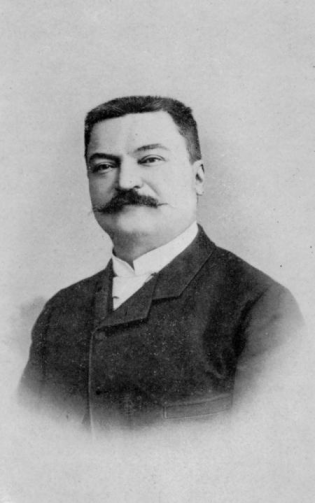
\includegraphics[width=1.5cm]{E_Lucas.png}\\
      \footnotesize{Édouard Lucas}
    \end{center}
  \end{frame}

  \begin{frame}{¿Qué es el cálculo umbral?}
      El objetivo era estudiar el comportamiento tan particular que ciertas sucesiones de números y polinomios poseen. 

      \begin{block}{\textbf{Idea fundacional}}
        \begin{align*}
        \text{Subíndices} & \leftrightarrow \text{Exponentes}\\
        a_0, a_1, \dots, a_n & \leftrightarrow a^0, a^1, \dots, a^n
        \end{align*}
      \end{block}
      La notación $a_k \equiv a^k$ se usa para simbolizar este intercambio. 
  \end{frame}

  \begin{frame}{El ejemplo clásico}
    Los números de Bernoulli $B_n$ suelen definirse a través de la función generadora
      \begin{equation*}
        \frac{x}{e^x - 1} = \sum_{n=0}^\infty B_n \frac{x^n}{n!}
      \end{equation*} 
      Con esta convención, podemos obtener lo siguiente
      \begin{align*}
        & e^{B \cdot x} = \sum_{n=0}^\infty B^n \frac{x^n}{n!} \equiv \sum_{n=0}^\infty B_n \frac{x^n}{n!} = \frac{x}{e^x - 1} \implies e^{B \cdot x} \equiv \frac{x}{e^x - 1}\\
        & \implies e^{-Bx} \equiv \frac{-x}{e^{-x}-1} = \frac{xe^x}{e^x-1} \equiv e^{(B+1) \cdot x} \implies (B+1)^n = (-B)^n
      \end{align*}
      Y de aquí se llega a la prueba del conocido resultado
      \begin{block}{}
        \begin{equation*}
        B_1 = -\frac{1}{2} \quad B_3 = B_5 = B_7 = \cdots = 0
      \end{equation*}
      \end{block}
  \end{frame}

  \begin{frame}{El ejemplo clásico}
    \begin{enumerate}
      \item Lo mismo se puede hacer con los polinomios de Bernoulli $B_n(x)$. 
      
      Su función generadora es
      \begin{equation*}
        \frac{zx}{e^{zx} - 1} = \sum_{n=0}^\infty B_n(x) \frac{z^n}{n!}
      \end{equation*}
      \item Otras tantas fórmulas conocidas apoyan esta idea.
      \begin{block}{}
        \begin{align*}
        &B_n(x + y) = \sum_{k=0}^n \binom{n}{k} B_{n-k}(y)x^k \leftrightarrow (x + y)^n = \sum_{k=0}^n \binom{n}{k} y^{n-k}x^k\\
        &B_n'(x) = nB_{n-1}(x) \leftrightarrow (x^n)' = nx^{n-1}\\
        &\int_{x}^{y} B_n(u) du = \frac{B_{n+1}(x) - B_{n+1}(y)}{n+1} \leftrightarrow \int_{x}^{y} u^n du = \frac{x^{n+1} - y^{n+1}}{n+1}
        \end{align*}
      \end{block}
    \end{enumerate}
  \end{frame}

  \begin{frame}
      \Large
      \begin{block}{}
        \begin{center}
          \textbf{¿A qué se deben estas aparentes coincidencias?}\\[1em]
          \textbf{¿Por qué funcionan estas manipulaciones?}\\[1em]
          \textbf{¿Se pueden generalizar los resultados a más sucesiones de polinomios?}
        \end{center}
      \end{block}
  \end{frame}

  \begin{frame}{El cálculo umbral moderno}
    \begin{block}{G-C. Rota, S.Roman}
      \begin{enumerate}
        \item Medio siglo después, revivirían todas estas ideas para darles la formalización necesaria y responder a estas preguntas.
        \item En 1984 publican \textbf{\textit{The Umbral Calculus}} que establece las bases de la disciplina.
      \end{enumerate}
    \end{block}
    \begin{center}
      \begin{minipage}{2.5cm}
        \centering
        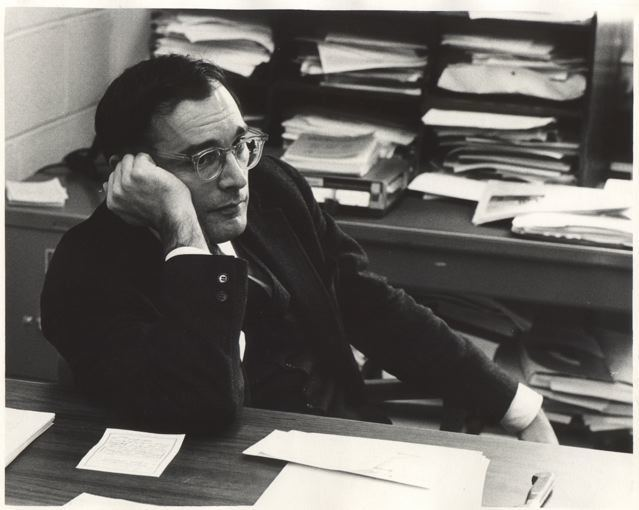
\includegraphics[width=3.1cm]{Rota.jpg}\\[1pt]
        \footnotesize Gian-Carlo Rota
      \end{minipage}
      \hspace{2.5cm}
      \begin{minipage}{2.5cm}
        \centering
        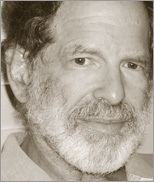
\includegraphics[width=2.2cm]{roman.jpeg}\\[1pt]
        \footnotesize Steven Roman
      \end{minipage}
    \end{center}
  \end{frame}

\begin{frame}{El cálculo umbral moderno}
  Todo se reduce al estudio y tratamiento de una clase especial de sucesiones de polinomios en 1 variable.

  \bigbreak \textbf{A grandes rasgos:}
\begin{center}
  \begin{tikzpicture}
    % Los tres recuadros de la izquierda
    \node[draw=darkred, fill=red!30, rounded corners=4pt,
          minimum width=4cm, minimum height=0.7cm,
          text centered] (sf) at (0, 4) {Series formales};
    
    \node[font=\small, text centered] (sf) at (0, 3) {+};

    \node[draw=darkred, fill=red!30, rounded corners=4pt,
          minimum width=4cm, minimum height=0.7cm,
          text centered] (af) at (0, 2) {Análisis funcional};

    \node[font=\small, text centered] (sf) at (0, 1) {+};

    \node[draw=darkred, fill=red!30, rounded corners=4pt,
          minimum width=4cm, minimum height=0.7cm,
          text centered] (al) at (0, 0) {Álgebra};

    % Recuadro destino a la derecha
    \node[draw=darkred, fill=red!30, rounded corners=4pt,
          minimum width=4cm, minimum height=0.7cm,
          text centered] (cu) at (6, 2) {Cálculo umbral moderno};

    % Línea vertical que agrupa los tres recuadros
    \draw[darkred] (2.2, 4) -- (2.2, 0);

    % Flecha desde el centro de la línea vertical al recuadro destino
    \draw[->, darkred, thick] (2.2, 2) -- (cu.west);
  \end{tikzpicture}
\end{center}
\end{frame}

\section{De series formales a funcionales y operadores}

  \begin{frame}{Definiciones y resultados previos}
    \begin{definicion}
      Se llama \textbf{funcional} a cada elemento de $\poly^*$, donde $\poly \equiv \field[x]$.
    \end{definicion}

    \begin{enumerate}
      \item Dado $L \in \poly^*$, $\langle L | p(x) \rangle$ simboliza su acción sobre el polinomio $p(x)$.
      \item Los funcionales están completamente determinados por una base; si $\{p_n(x)\}_{n\geq0}$ es una base de $\poly$, entonces las constantes $\langle L | p_n(x) \rangle$ definen al funcional.
      \item En particular, todas las sucesiones $\{p_n(x)\}_{n\geq0}$ tales que $\gr(p_n) = n$ para todo $n$ determinan a los funcionales.
    \end{enumerate}
    \begin{block}{}
      Concretamente, los escalares $\{\langle L | x^n \rangle \}_{n \geq 0}$ determinan por completo a los funcionales.
    \end{block}
  \end{frame}

  \begin{frame}{Series formales como funcionales}
    En consecuencia, podemos definir las asignaciones siguientes:
    \begin{enumerate}
      \item $T^k \longrightarrow \omega_{T^k} \text{ con } \langle \omega_{T^k} | x^n \rangle = n! \cdot \delta_{n,k}$. 
      
      Por linealidad, $F(T) \longrightarrow \omega_{F}$ con $\rboxed{\langle \omega_F | x^n \rangle = n! \cdot a_n}$.
      \item $L \longrightarrow F_L(T)$ con $\rboxed{F_L(T) = \displaystyle \sum_{k=0}^\infty \frac{ \langle L | x^k \rangle}{k!} T^k }$
    \end{enumerate}
  \end{frame}

  \begin{frame}{Series formales como funcionales}
    \begin{teorema}[(isomorfismo canónico umbral)]
      La aplicación $\phi \colon  \poly^* \xrightarrow{\sim} \F$ definida por
    \begin{align*}
        L & \mapsto F_L(T) = \sum_{k=0}^\infty \frac{ \langle L | x^k \rangle}{k!} T^k \quad \quad \omega_F \mapsfrom F(T) = \sum_{k=0}^\infty a_k T^k
    \end{align*}
    es un isomorfismo lineal.
    \end{teorema}
  \end{frame}

  \begin{frame}{El álgebra umbral}
    $\phi$ \underline{no} es isomorfismo de álgebras (con la estructura clásica). Un nuevo producto aparece en $\poly^*$:
    \begin{align*}
      \phi(L) \cdot \phi(M) & = \left(\sum_{k=0}^\infty \frac{\langle L | x^k \rangle}{k!}T^k\right) \cdot \left(\sum_{r=0}^\infty \frac{\langle M | x^r \rangle}{r!}T^r\right) \\
      & = \sum_{n = 0}^\infty \left( \sum_{k=0}^{n} \frac{\langle L | x^k\rangle}{k!} \cdot \frac{\langle M | x^{n-k} \rangle}{(n-k)!}\right) T^n\\
      & = \sum_{n = 0}^\infty \frac{1}{n!} \left( \sum_{k=0}^{n} \binom{n}{k} \langle L | x^k\rangle \langle M | x^{n-k} \rangle\right) T^n
    \end{align*}
  \end{frame}

  \begin{frame}{El álgebra umbral}
    \begin{definicion}
      Se llama \textbf{álgebra umbral} al espacio vectorial $\poly^*$ dotado de la estructura de $\field$-álgebra inducida por $\phi$, es decir, aquella definida por
        \begin{equation*}
        \langle L \cdot M | x^n \rangle = \sum_{k=0}^n \binom{n}{k}\langle L | x^k \rangle \langle M | x^{n-k} \rangle \quad \forall L, M \in \poly^*
        \end{equation*} 
    \end{definicion}
    En particular, cumple que
    \begin{enumerate}
      \item $e^{0T} = 1$ es la identidad para el producto del álgebra umbral.
      \item $\displaystyle \langle L_1 \cdots L_m | x^n \rangle = \sum_{|i|=n}\binom{n}{i_1, \dots , i_m} \langle L_1| x^{i_1} \rangle \dots  \langle L_m | x^{i_m} \rangle$ donde $|i| = i_1 + \dots +i_m$ y $\binom{n}{i_1, \dots , i_m} = \frac{n!}{k_1! \cdots k_m!}$
    \end{enumerate}
  \end{frame}

  \begin{frame}{El álgebra umbral}
    Ahora, $\phi$ será un isomorfismo de álgebras entre esta nueva álgebra umbral y el álgebra formal. En particular
    \begin{equation*}
      F(T) = G(T) \iff \phi^{-1}(F(T)) = \phi^{-1}(G(T)) \iff \omega_F = \omega_G
    \end{equation*}

    \begin{block}{Notación}
      $F(T)$ simbolizará a la serie formal y al funcional $\omega_F$ asociado.
      \begin{align*}
        F(T) \equiv \omega_F & \colon \poly \longrightarrow \field \\
        & p(x) \mapsto \langle F(T)| p(x)\rangle
      \end{align*}
    \end{block}
  \end{frame}

  \begin{frame}{Algunos ejemplos}
    \begin{enumerate}
      \item \textbf{Funcionales derivada k-ésima}
      \begin{align*}
        \langle T^k| x^n \rangle = n! \cdot \delta_{n,k} = (x^n)^{(k)}(0) \implies
          \rboxed{\langle T^k| p(x) \rangle = p^{(k)}(0)}
      \end{align*}
      \item \textbf{Funcional evaluación en $\lambda$}. Simbolizamos por $E_{\lambda}$ a la serie  $e^{\lambda T}$
      \begin{align*}
        \langle E_{\lambda} | x^n \rangle = \left\langle \sum_{k = 0}^\infty \frac{\lambda^k}{k!}T^k | x^n \right\rangle = n! \cdot \frac{\lambda^n}{n!} = \lambda^n \implies \rboxed{\langle E_{\lambda} | p(x) \rangle = p(\lambda)}
      \end{align*}
      \item \textbf{Funcional diferencia con $\lambda$}. Simbolizamos por $\Delta_{\lambda}$ a la serie $E_{\lambda} - 1$
      \begin{align*}
        \rboxed{\langle \Delta_{\lambda} | p(x) \rangle = \langle e^{\lambda T}-1 | p(x) \rangle = p(\lambda)-p(0)} 
      \end{align*}
      \item \textbf{Funcional de Abel en $\lambda$}
      \begin{align*}
        \langle T E_\lambda | x^n \rangle = \left\langle \sum_{n\geq0} \frac{\lambda^n}{n!}T^{n+1} | x^n \right\rangle = nx^{n-1} \implies \rboxed{\langle Te^{\lambda T} | p(x) \rangle = p^`(\lambda)}
      \end{align*}
    \end{enumerate}
  \end{frame}

  \begin{frame}{Propiedades de las series como funcionales}
    \begin{proposicion}[(desarrollos de Taylor)]
    Sean $F(T) \in \F$ y $p(x) \in \poly$. Se tiene que
    \begin{enumerate}
        \item $\begin{aligned}[t]
            F(T) = \sum_{k = 0}^\infty \frac{ \langle F(T) | x^k \rangle}{k!}T^k \quad \text{\textbf{(Taylor para funcionales)}}
        \end{aligned}$ 
        \item $\begin{aligned}
            p(x) = \sum_{k \geq 0} \frac{ \langle T^k| p(x) \rangle}{k!}x^k \quad \text{\textbf{(Taylor clásico)}}
        \end{aligned}$
    \end{enumerate}
  \end{proposicion}

  \begin{demo}
    La segunda igualdad solo es una reescritura del teorema de Taylor habitual para polinomios. La primera es consecuencia directa de la definición del funcional $F(T)$ pues $\langle F(T) | x^k\rangle = k! \cdot a_k$.
  \end{demo}
\end{frame}

\begin{frame}{Propiedades de las series como funcionales}
  \begin{proposicion}[(adjunción de derivada formal)]
      \begin{equation*}
        \langle \partial F(T) | p(x) \rangle = \langle F(T) | x \cdot p(x)\rangle \quad \forall F(T) \in \F, p(x) \in \poly
      \end{equation*}
    \end{proposicion}
    \begin{demo}
      Por la linealidad, basta verlo para $p(x) = x^n$. En ese caso 
        \begin{align*}
            \langle \partial F(T)| x^n\rangle & = \sum_{k=1}^\infty ka_k\langle T^{k-1}| x^n\rangle = \sum_{k=0}^\infty (k+1)a_{k+1}\langle T^{k}| x^n\rangle \\
            & = \sum_{k=0}^\infty (k+1)a_{k+1}k! \delta_{n,k} = (n+1)!a_{n+1}\\ 
            & = \langle F(T)| x^{n+1}\rangle = \langle F(T)| x\cdot x^n\rangle \qedhere
        \end{align*}
    \end{demo}
\end{frame}

\begin{frame}{Series como operadores}
  \begin{definicion}
    Llamaremos \textbf{operador} a cada elemento de $\End(\poly)$. Además, dado operador $\Lambda \in \poly^*$ simbolizaremos su acción sobre un polinomio $p(x)$ simplemente como $\Lambda p(x)$.
  \end{definicion}
  \begin{enumerate}
    \item Como con los funcionales, podemos asignar la variable formal $T$ a la derivada formal: $T \mapsto \partial_{x}$.
    \item Por linealidad, se extiende a la aplicación $\varphi$ siguiente:
  \end{enumerate}
  \begin{block}{}
    \begin{align*}
      \varphi \colon \F & \longrightarrow \End(\poly)\\
      \sum_{k = 0}^\infty \frac{a_k}{k!}T^k & \mapsto \sum_{k = 0}^\infty \frac{a_k}{k!} \partial_{x}^k = \varphi(F(T))
    \end{align*}
  \end{block}
\end{frame}

\begin{frame}{$\poly$ como $\F$-módulo}
  \begin{block}{Notación}
    $F(T)$ simbolizará también al funcional asociado $\varphi(F(T))$.
    \begin{align*}
    F(T) \equiv \varphi(F(T)) \colon & \poly \longrightarrow \poly \nonumber \\
    & x^n \mapsto F(T)x^n = \sum_{k=0}^n \binom{n}{k}a_k x^{n-k}
    \end{align*}
  \end{block}

  \begin{enumerate}
    \item Se verifica que $\varphi$ \textbf{es un morfismo de álgebras}, es decir, se verifica que $\varphi(F(T) \cdot G(T)) = \varphi(F(T)) \circ \varphi(G(T))$
    \item Con esta notación, esto se corresponde con que
      \begin{equation*}
        \rboxed{F(T) \cdot G(T) = F(T) \circ G(T)}
      \end{equation*}
  \end{enumerate}
\end{frame}

\begin{frame}{$\poly$ como $\F$-módulo}
  En particular, esto se traduce en que $\poly$ es un $\F$-módulo 
  \begin{teorema}[(estructura de módulo)]
    El producto definido por
    \begin{align*}
        \star \colon & \F \times \poly \longrightarrow \poly\\
        & (F(T), p(x)) \mapsto F(T) \star p(x) \equiv F(T) p(x)
    \end{align*}
    dota a $\poly$ de una estructura de $\F$-módulo. Además, es un módulo \textbf{fiel}.
  \end{teorema}
  \begin{block}{}
    En este caso, $\varphi$ \textbf{no es una biyección} pues no es epiyectiva; existen operadores $\Lambda$ que no se corresponden con niguna serie formal.
  \end{block}
\end{frame}

\begin{frame}{Series, operadores y funcionales}
  \textbf{En resumen, $F(T)$ simboliza tres objetos distintos:}

  \begin{center}
  \begin{tikzpicture}[
    box/.style={
        draw=red!70!black, thick, rounded corners,
        fill=red!25,
        minimum width=3cm, minimum height=1.8cm,
        align=center, font=\small, inner sep=4pt
    },
    arrowstyle/.style={<->, >=Latex, thick}
]

% Caja superior (centrada)
\node[box] (A) at (0,2.2) {
    \textbf{Serie formal}\\[4pt]
    $\displaystyle F(T)=\sum_{k=0}^{\infty}\frac{a_k}{k!}T^k$
};

% Cajas inferiores (simétricas respecto al eje vertical de A)
\node[box] (B) at (-3.2,0) {
    \textbf{Funcional}\\[4pt]
    $\displaystyle \langle F(T)|x^n\rangle = a_n$
};

\node[box] (C) at (3.2,0) {
    \textbf{Operador}\\[4pt]
    $\displaystyle F(T)x^n=\sum_{k=0}^{n}\binom{n}{k}a_kx^k$
};

% Flechas saliendo ambas de la caja superior
\draw[arrowstyle] (-1.5, 2) -- (B.north);
\draw[->] (1.5, 2) -- (C.north);

\end{tikzpicture}
\end{center}

\end{frame}

\begin{frame}{Operadores con forma de serie formal}
  \begin{enumerate}
      \item \textbf{Operadores derivada k-ésima}, $T^k$:
        \begin{equation*}
          \rboxed{T^k p(x) = p^{(k)}(x)}        
        \end{equation*}
      \item \textbf{Operador traslación con $\lambda$}, $E_{\lambda}$:
        \begin{equation*}
            E_{\lambda} x^n = \sum_{k=0}^\infty \frac{\lambda^k}{k!} T^kx^n = (x+ \lambda )^n \implies \rboxed{E_{\lambda} p(x) = p(x+\lambda)}
        \end{equation*} 
      \item \textbf{Operador diferencia con $\lambda$}, $\Delta_{\lambda}$:
      \begin{equation*}
        \rboxed{\Delta_{\lambda} p(x) = p(x+ \lambda) - p(x)}
      \end{equation*}
      \item \textbf{Operador de Abel en $\lambda$}, $TE_{\lambda}$:
      \begin{equation*}
        \rboxed{TE_{\lambda}p(x) = p'(x+ \lambda)}
      \end{equation*}
    \end{enumerate}
\end{frame}

\begin{frame}{Operadores con forma de serie formal}
  \begin{enumerate}[5]
    \item Otro ejemplo importante es el operador $\frac{\Delta_{\lambda}}{T}$
      \begin{align*}
          \frac{\Delta_{\lambda}}{T}x^n & = \left(\sum_{k=0}^\infty \frac{\lambda^{k+1}}{(k+1)!}T^k\right) x^n = \sum_{k=0}^n \binom{n+1}{k+1} \frac{\lambda^{k+1}}{(n+1)}x^{n-k}\\
          & = \frac{1}{n+1}\sum_{k=1}^{n+1} \binom{n+1}{k} \lambda^k x^{n+1-k} = \frac{1}{n+1}((x+ \lambda )^{n+1} - x^{n+1})\\ 
          & = \int\limits_{x}^{x+ \lambda} u^n \, du
      \end{align*}
        Por tanto, para un polinomio genérico $p(x)$
        \begin{equation*}
          \rboxed{\displaystyle \frac{\Delta_{\lambda}}{T}p(x) = \int\limits_{x}^{x+ \lambda} p(u) \, du}
        \end{equation*}
  \end{enumerate}
\end{frame}

\begin{frame}[fragile]{Relación entre operadores y funcionales}
  \begin{teorema}[(adjunción operadores y funcionales)]
    Sean $F(T), G(T) \in \F$ y $p(x) \in \poly$. Entonces
    \begin{equation*}
        \langle F(T) \cdot G(T) | p(x) \rangle = \langle F(T) | G(T)p(x) \rangle 
    \end{equation*}
  \end{teorema}

  \begin{demo}
    Por linealidad, se reduce al caso trivial de las series $T^k$
  \end{demo}
\end{frame}

\section{Sucesiones de Sheffer}

  \begin{frame}{Series delta e invertibles}
    \begin{definicion}
      Una serie formal $F(T)$ es una \textbf{serie delta} (o \textbf{$\delta$-serie}) si $F(T)$ es un invertible respecto de la composición formal. 
      
      % Creamos un punto de anclaje perfectamente centrado abajo
      \centering\tikzmark{A}
    \end{definicion}

    \vspace{0.5cm}

    \begin{definicion}
      % Creamos un punto de anclaje perfectamente centrado arriba
      \centering\tikzmark{B}\flushleft
      Un funcional $L \in \poly^*$ es un \textbf{funcional delta} (o \textbf{$\delta$-funcional}) si como serie es una serie delta y es un \textbf{funcional invertible} si como serie es una serie invertible. Análogamente, un operador $F(T) \in \text{Im}(\varphi)$ es un \textbf{operador delta} (o \textbf{$\delta$-operador}) si como serie es una serie delta y es un \textbf{operador invertible} si como serie es una serie invertible. 
    \end{definicion}
    
    % Dibujamos la flecha negra y perfectamente vertical
    \begin{tikzpicture}[remember picture, overlay]
        \draw[-{Stealth[scale=1.5]}, line width=1.5pt, black!50] 
            ([yshift=-4mm]pic cs:A) -- ([yshift=+9mm]pic cs:B);
    \end{tikzpicture}
  \end{frame}

  \begin{frame}{Sucesiones de Sheffer}
    \begin{enumerate}
      \item Por construcción, ya sabemos que $\langle T^k | x^n\rangle = n! \cdot \delta_{n,k}$
      \item Buscamos responder a la pregunta siguiente:\\
      \begin{center}
        \textbf{¿se puede generalizar este hecho?}
      \end{center}
      \begin{block}{}
        Es decir, encontrar serie $H(T)$ y sucesión $\{r_n(x)\}_{n \geq 0}$ tales que 
        \begin{equation*}
          \langle H^k(T) | r_n(x) \rangle = n! \cdot \delta_{n,k}
        \end{equation*}
      \end{block}
    \end{enumerate}
  \end{frame}

  \begin{frame}{Sucesiones de Sheffer}
    \begin{teorema}[(de existencia de las sucesiones de Sheffer)]
      Sea $F(T) \in \F^{\delta}$ una serie delta y $G(T) \in \F^*$ una serie invertible. Existe una \textbf{única} sucesion de polinomios $s_n(x)$ con $\gr(s_n) = n$ tal que para todo entero $k \geq 0$ verifica que
      \begin{equation*}
        \langle G(T)F^k(T)| s_n(x) \rangle = n! \cdot \delta_{n,k}
      \end{equation*}
    \end{teorema}
  \end{frame}

  \begin{frame}{Sucesiones de Sheffer}
    \begin{definicion}
      \begin{enumerate}
        \item Se llama \textbf{sucesión de Sheffer asociada a $(¡G(T), F(T))$} a la sucesión de polinomios $s_n(x)$ anterior. Se simboliza por la notación $s_n(x) \sim (G(T), F(T))$ y $\Sh$ es el conjunto de estas sucesiones. 
        \item En particular, Si $F(T) = T$ decimos que $s_n(x)$ es la \textbf{sucesión de Appell asociada a $G(T)$} y si $G(T) = 1$ decimos que $p_n(x)$ es la \textbf{sucesión asociada a $F(T)$}. Escribiremos $p_n(x) \sim F(T)$ para indicar que esta es la sucesión asociada a $F(T)$ y $\Umb$ y $\App$ simbolizarán los conjuntos de las sucesiones asociadas y de Appell, respectivamente.
      \end{enumerate}
    \end{definicion}
  \end{frame}

  \begin{frame}{Sucesiones de Sheffer}
      \begin{enumerate}
        \item \textbf{Ejemplo:} $x^n \sim T$ puesto que $\langle T^k| x^n\rangle = n! \cdot \delta_{n,k}$.
        \item \textbf{Ejemplo:} Por inducción, uno puede ver que $(x)_n = x(x-1)\cdots (x-n+1) \sim \Delta$
      \end{enumerate}

      \begin{proposicion}
        $s_n(x) \sim (G(T), F(T)) \iff p_n(x) = G(T)s_n(x) \sim F(T)$
      \end{proposicion}

      \begin{demo}
        $\langle F^k(T) | G(T)s_n(x) \rangle = \langle F^k(T)G(T) | s_n(x) \rangle = n! \cdot \delta_{n,k}$
      \end{demo}
  \end{frame}

  \begin{frame}{Comportamiento de estas sucesiones}
    Es natural entonces preguntarse si las sucesiones de Sheffer generalizan más comportamientos de las potencias $x^n$. 
      \begin{block}{}
        \begin{align*}
          p(x) = \sum_{k \geq 0} \frac{p^{(k)}(0)}{k!}x^k \leftrightarrow p(x) = \sum_{k \geq 0} a_k s_k(x) \text{ con } a_k = \text{ ?}\\
          (x+y)^n = \sum_{k=0}^{n} \binom{n}{k} x^k y^{n-k} \leftrightarrow s_n(x+y) = \text{ ?} \\
          Tx^n = (x^n)' = nx^{n-1} \leftrightarrow F(T)s_n(x) = \text{ ?}
        \end{align*}
      \end{block}
  \end{frame}

  \begin{frame}{Los teoremas de expansión}
    \begin{teorema}[(de expansión para series formales)]
      Sea $s_n(x) \sim (G(T), F(T))$. Entonces
      \begin{equation*}
        H(T) = \sum_{k = 0}^\infty \frac{\langle H(T)| s_k(x)\rangle}{k!}G(T)F^k(T) \quad \forall H(T) \in \F
      \end{equation*}
    \end{teorema}

    \begin{teorema}[(de expansión para polinomios)]
      Sea $s_n(x) \sim (G(T), F(T))$. Entonces
      \begin{equation*}
        p(x) = \sum_{k \geq 0} \frac{\langle G(T)F^k(T) | p(x) \rangle}{k!}s_k(x) \quad \forall p(x) \in \poly
      \end{equation*}
    \end{teorema}
  \end{frame}

  \begin{frame}{Caracterizaciones}
    \begin{teorema}[(función generadora)]
      \begin{align*}
        s_n(x) \sim (G(T), F(T)) \iff \frac{1}{G(F^{-1}(T))}E_{\xi} (F^{-1}(T)) = & \sum_{k=0}^\infty \frac{s_k(\xi)}{k!}T^k \\ 
        & \forall \xi \in \field
      \end{align*}
    \end{teorema}

    \begin{demo}
      Si $s_n(x) \sim (G(T), F(T))$, entonces la serie $E_{\xi}$ es\\
      \small{$\displaystyle E_{\xi}(T) = \sum_{k=0}^\infty \frac{s_k(\xi)}{k!}G(T)F^k(T)$}. Despejando se llega al resultado.

      Recíprocamente, si $r_n(x) \sim (G(T), F(T))$, entonces hemos visto que se da la igualdad del enunciado para $r_n(x)$. Con lo que $r_n(\xi) = s_n(\xi)$ y se concluye.
    \end{demo}
  \end{frame}

  \begin{frame}{Caracterizaciones}
    \begin{teorema}[(caracterización diferencial)]
      \begin{equation*}
        s_n(x) \sim (G(T), F(T)) \iff F(T)s_{n}(x) = ns_{n-1}(x) \quad \forall n \geq 0
      \end{equation*}
    \end{teorema}

    \begin{teorema}[(identidad de Sheffer)]
      Sea $p_n(x) \sim F(T)$. Entonces
      \begin{equation*}
        s_n(x) \sim (G(T), F(T)) \iff s_n (x+y) = \sum_{k=0}^n \binom{n}{k} p_k (y) s_{n-k}(x)
      \end{equation*}
    \end{teorema}
  \end{frame}

\begin{frame}{Operadores adjuntos}
  \begin{definicion}
    Dado un operador $\Lambda \in \End(\poly)$ llamaremos \textbf{operador adjunto de $\Lambda$} al operador lineal $\Lambda^* \in \End(\poly^*)$ tal que para cada $p(x) \in \poly$
    \begin{equation*}
        \langle \Lambda^* F(T) | p(x) \rangle = \langle F(T) | \Lambda p(x) \rangle
    \end{equation*}
  \end{definicion}
\end{frame}

\begin{frame}{Ejemplos de operadores adjuntos}
\begin{definicion}
  \begin{enumerate}
    \item Se define el \textbf{operador multiplicación asociado a $F(T)$} como el operador lineal $M^*(F) \in \End(\poly^*)$ que viene definido por $G(T) \mapsto F(T) \cdot G(T)$
    \item Se define el \textbf{operador multiplicación por x} como el operador $M \in \End(\poly)$ que viene definido por $p(x) \mapsto x \cdot p(x)$
  \end{enumerate}
  
\end{definicion}
  \textbf{Ejemplos:}
  \begin{enumerate}
      \item $\langle F(T) \cdot G(T) | p(x) \rangle = \langle G(T) | F(T)p(x) \rangle \implies \rboxed{F(T)^* = M^*(F)}$
      \item $\langle \partial F(T) | p(x) \rangle = \langle F(T) | x \cdot p(x)\rangle \implies \rboxed{M^* = \partial}$
    \end{enumerate}
\end{frame}

\begin{frame}{Operadores de Sheffer}
  \begin{definicion}
    Dada $s_n(x) \sim (G(T), F(T))$, se llama \textbf{operador de Sheffer asociado a $s_n(x)$ o a $(G(T), F(T))$} al operador $\Lambda_{G,F} \in \End(\poly)$ dado por
    \begin{equation*}
        \Lambda_{G,F} x^n = s_n(x)
    \end{equation*}
    En el caso de que $p_n(x)$ sea la sucesión asociada a $F(T)$ decimos que $\Lambda_{1, F} \equiv \Lambda_{F}$ es simplemente el \textbf{operador umbral asociado a $p_n(x) $ o a $F(T)$} y se simbolizarán a ambos conjuntos por $\End_{\mathrm{Sh}}(\poly)$ y $\End_{\mathrm{Umb}}(\poly)$, respectivamente.
  \end{definicion}
\end{frame}

\begin{frame}{Operadores de Sheffer}
  \begin{proposicion}
     Dado $\Lambda_{G,F} \in \End_{\mathrm{Sh}}(\poly)$ se verifica que $\Lambda_{G,F} = \frac{1}{G(T)} \circ \Lambda_{F}$
  \end{proposicion}

  \begin{demo}
    $\displaystyle s_n(x) \sim (G(T), F(T)) \implies p_n(x) = G(T)s_n(x) \sim F(T)$
    \bigbreak
    $\displaystyle \implies \Lambda_{G,F}x^n = s_n(x) = \frac{1}{G(T)} p_n(x) = \left(\frac{1}{G(T)} \circ \Lambda_{F}\right) x^n$
    \bigbreak
    $\displaystyle \implies \Lambda_{G,F} = \frac{1}{G(T)} \circ \Lambda_{F} \qedhere$
  \end{demo}

  \begin{block}{Corolario}
      Teoría de $\End_{\mathrm{Umb}}(\poly) \implies$ Teoría de $\End_{\mathrm{Sh}}(\poly)$
  \end{block}
\end{frame}

\begin{frame}{Operadores de Sheffer}
  \begin{teorema}[(caracterización operadores umbrales)]
    Se tiene la igualdad de conjuntos $\mu_{\mathcal{C}}^{-1}(\Aut(\poly^*)) = \End_{umb}(\poly)$. Además, para todo operador umbral $\Lambda_F \in \End_{umb}(\poly)$ y todo funcional $G(T) \in \poly^*$ se verifica que
    \begin{equation*}
        \Lambda_F^*G(T) = G(F^{-1}(T))
    \end{equation*}
  \end{teorema}

  \begin{enumerate}
    \item Como corolario, se tiene que $\mu_{\mathcal{C}}(\End_{\mathrm{Sh}}(\poly)) = \Aut(\poly^*) \cup M^*(\poly^*)$
    \item Además, se tiene que 
      \begin{block}{}
        \begin{equation*}
          \Lambda_{G,F}^*H(T) = \frac{1}{G(F^{-1}(T))} H(F^{-1}(T)) 
        \end{equation*}
      \end{block}
  \end{enumerate}
\end{frame}

\begin{frame}{Operadores de Sheffer}
  
  \begin{teorema}
    $\End_{\mathrm{Umb}}(\poly)$ es un grupo bajo la ley de grupo dada por la composición de aplicaciones. Concretamente $\Lambda_F \circ \Lambda_G = \Lambda_{G \circ F} \text{ y } \Lambda_F^{-1} = \Lambda_{F^{-1}}$
  \end{teorema}

  \begin{demo}
    \begin{align*}
        (\Lambda_F \circ \Lambda_G)^*H(T) = \Lambda_G^* H(F^{-1}(T)) = H(F^{-1}(G^{-1}(T))) & = H((G \circ F)^{-1}(T)) \\
        & = \Lambda_{G \circ F}^*H(T)
    \end{align*}
    \begin{align*}
      \implies (\Lambda_F \circ \Lambda_G)^* = \Lambda_{G \circ F}^* \implies \Lambda_F \circ \Lambda_G = \Lambda_{G \circ F}
    \end{align*}
    De igual forma se ve para $\Lambda_F^{-1}$.
  \end{demo}
  \begin{block}{}
    \begin{enumerate}
      \item Como corolario, $\End_{\mathrm{Sh}}(\poly)$ es también un grupo con la composición.
      \item Concretamente, $\Lambda_{G,F} \circ \Lambda_{H,L} = \Lambda_{G \cdot H \circ F, L \circ F} \text{ y } \Lambda_{G, F}^{-1} = \Lambda_{1/(G   \circ F^{-1}), F^{-1}}$
    \end{enumerate}
  \end{block}
\end{frame}

\begin{frame}{Composición umbral}
  \begin{definicion}
    Dadas $s_n(x) \sim (G(T), F(T))$ y $r_n(x) \sim (H(T), L(T))$ se define la $\textbf{composición umbral}$ de $r_n(x) = \displaystyle \sum_{k=0}^n r_{n,k}x^k$ con $s_n(x)$ como
    \begin{equation*}
        r_n(\mbox{\bfseries s(x)}) = \sum_{k=0}^n r_{n,k}s_k(x)
    \end{equation*} 
\end{definicion}
Los operadores de Sheffer definen la composición umbral
  \begin{align*}
    \Lambda_{G,F}r_n(x) & = \Lambda_{G,F} \left[\sum_{k=0}^n r_{n,k}x^k \right] = \sum_{k=0}^n r_{n,k}s_k(x)\\
    \implies & \rboxed{r_n(\mbox{\bfseries s(x)}) = \Lambda_{G,F}r_n(x)}
  \end{align*}
\end{frame}

\begin{frame}{Composición umbral}
  Es natural entonces pensar que tendremos estructura de grupo en $\Sh$.
  \begin{teorema}
    $\Sh$ es un grupo con la ley de grupo dada por la composición umbral. En particular
    \begin{enumerate}
        \item Si $s_n(x) \sim (G(T), F(T))$ y  $r_n(x) \sim (H(T), L(T))$, entonces la sucesión de la composición umbral es $r_n(\mathbf{s(x)}) \sim (G(T)H(F(T)), L(F(T)))$ 
        \item $x^n$ es la identidad 
        \item Si $s_n(x) \sim (G(T), F(T))$,entonces $s_n^{-1}(x) = q_n(x)$ para $q_n(x) \sim (G(F^{-1}(T)), F^{-1}(T))$
    \end{enumerate}
  \end{teorema}
\end{frame}
  
\section{Aplicaciones de toda esta teoría}

\subsection{Los polinomios de Bernoulli}
  \begin{frame}{Los polinomios de Bernoulli}
    \begin{definicion}
      Se llaman \textbf{polinomios de Bernoulli de orden $r$} a los polinomios $B_n^{(r)}(x)$ que forman la sucesión de Appell para
    \begin{equation*}
        G(T) \equiv \left(\frac{e^T - 1}{T}\right)^r \equiv \left(\frac{\Delta}{T}\right)^r \quad \text{ con } r \in \field^*
    \end{equation*}
    Para $r = 1$, se llaman solo \textbf{polinomios de Bernoulli} y son $B_n(x)$.
    \end{definicion}

    \begin{definicion}
    Se llaman \textbf{números de Bernoulli de orden $r$} a los escalares $B_n^{(r)}(0)$ y se simbolizan como $B_n^{(r)}$. Si $r=1$, se llaman simplemente \textbf{números de Bernoulli} y se escriben como $B_n$.
\end{definicion}
\end{frame}

\begin{frame}{Los polinomios de Bernoulli}
  Los números de Bernoulli aparecen en multitud de áreas matemáticas.
  Fundamental es su relación con la \textbf{función zeta de Riemann}:
  \begin{block}{}
    \begin{equation*}
      \zeta(2k) = (-1)^{k-1}B_{2k}\frac{2^{2k-1}}{(2k)!}\pi^{2k}
    \end{equation*}
  \end{block}
  Incluso, para la más general \textbf{función zeta de Hurtwiz} $ \zeta(s, r) = \sum_{n} \frac{1}{(n+r)^s}$:
  \begin{block}{}
    \begin{equation*}
      \zeta (-n, a) = -\frac{B_{n+1}(a)}{n+1} \implies \zeta (-n) = - \frac{B_{n+1}}{n+1}
    \end{equation*}
  \end{block}
\end{frame}

\begin{frame}{Los polinomios de Bernoulli}
  Varios resultados conocidos se vuelven inmediatos.
  \begin{enumerate}
    \item \textbf{Caracterización diferencial:} $F(T)s_{n}(x) = ns_{n-1}(x)$ \begin{equation*}
      \implies \rboxed{\left(B_n^{(r)}(x)\right)' = n B_{n-1}^{(r)}(x)}
    \end{equation*}
    \item \textbf{Función generadora:} $\frac{1}{G(F^{-1}(T))}E_{\xi} (F^{-1}(T)) = \sum_{k=0}^\infty \frac{s_k(\xi)}{k!}T^k$ \begin{equation*}
      \implies \rboxed{\displaystyle \sum_{k=0}^\infty \frac{B_k^{(r)}(x)}{k!} T^k = \left(\frac{T}{e^T - 1}\right)^r e^{x T}}
    \end{equation*}
    \item \textbf{Identidad de Appell:} $s_n (x+y) = \sum_{k=0}^n \binom{n}{k} s_k (y) x^{n-k}$ \begin{equation*}
      \implies \rboxed{\displaystyle B_n^{(r)}(x + y) = \sum_{k=0}^n \binom{n}{k} B_k^{(r)}(y)x^{n-k}}
    \end{equation*}
  \end{enumerate}
\end{frame}

\begin{frame}{Los polinomios de Bernoulli}
  \begin{block}{Caracterización integral}
    \begin{equation*}
        \int_{x}^{x + y} B_n^{(r)}(u) du = \frac{B_{n+1}^{(r)}(x + y) - B_{n+1}^{(r)}(x)}{n+1}, \forall x, y \in \field
    \end{equation*}
  \end{block}

  \begin{demo}
    \begin{align*}
        & \int_{x}^{x + y} B_n^{(r)}(u) du = \left(\frac{\Delta_y}{T}\right) B_n^{(r)}(x) = \sum_{k=1}^{\infty} \frac{y^k}{k!} T^{k-1}B_{n}^{(r)}(x)\\ 
        & \stackrel{\scriptsize{\text{Car. Dif}}}{=} \sum_{k=1}^{n+1} \frac{y^k}{k!} (n)_{k-1}B_{(n+1) - k}^{(r)}(x) = \frac{1}{n+1} \sum_{k=1}^{n+1} \binom{n+1}{k} y^k B_{(n+1) - k}^{(r)}(x)\\
        & \stackrel{\scriptsize \text{Id. Appell}}{=} \frac{1}{n+1} (B_{n+1}^{(r)}(x + y) - B_{n+1}^{(r)}(x)) \qedhere
    \end{align*}
  \end{demo}
\end{frame}

\begin{frame}{Los polinomios de Bernoulli}
  \begin{block}{Ecuación de recurrencia de orden $r$}
    \begin{enumerate}
      \item $\displaystyle B_n^{(r)}(x +1) = B_n^{(r)}(x) + nB_{n-1}^{(r-1)}(x), (r \neq 1)$
      \item $\displaystyle B_n(x+1) = B_n(x) + nx^{n-1}$
    \end{enumerate}
  \end{block}

  \begin{demo}
    Basta usar que $p_n(x) = G(T)s_n(x)$, que se traduce a que $B_n^{(r)}(x) = (\frac{T}{\Delta})^r x^n$:
    \small{$ \displaystyle B_n^{(r)}(x+1) - B_n^{(r)}(x) = \Delta B_n^{(r)}(x) = \Delta \left(\frac{T}{\Delta}\right)^r x^n = \left(\frac{T}{\Delta}\right)^{r-1} T x^n = nB_{n-1}^{(r-1)}(x)$}. El mismo razonamiento aplica para el caso 2.
  \end{demo}
\end{frame}

\begin{frame}{Los polinomios de Bernoulli}
  \begin{teorema}[(sumación de Euler-Maclaurin para polinomios)]
    Dado $p(x) \in \poly$ se verifica que
    \begin{equation*}
        \sum_{i=0}^{m-1} p(n+i) = \int_{n}^{n + m} p(u)du + \sum_{k = 1}^\infty \frac{B_k}{k!}\left(p^{(k-1)}(n + m) - p^{(k-1)}(n) \right)
    \end{equation*}
    para todo $n, m \in \Z \text{ tal que } n < m$
  \end{teorema}
\end{frame}

\begin{frame}{Los polinomios de Bernoulli}
  \begin{demo}
    El teorema de expansión aplicado a la traslación $E_y$ con los polinomios de Bernoulli da que
    \begin{equation*}
        E_y(T) = \frac{\Delta}{T} + \sum_{k=1}^\infty \frac{B_k(y)}{k!} (e^T - 1) T^{k-1} 
    \end{equation*}
    Aplicado a un polinomio genérico $p(x) \in \poly$ esto es
    \begin{equation*}
        p(x+y) = \int_{x}^{x+1} p(u)du + \sum_{k=1}^\infty \frac{B_k(y)}{k!} \left(p^{(k-1)}(x+1) - p^{(k-1)}(x)\right)
    \end{equation*}
    Con $y = 0$ y $x = n, n + 1, \dots, n + m -1$, llegamos a las $m$ ecuaciones:
    \begin{equation*}
        p(n + i) = \int_{n+i}^{n + i + 1} p(u)du + \sum_{k=1}^\infty \frac{B_k}{k!} \left(p^{(k-1)}(n + i + 1) - p^{(k-1)}(n + i)\right)
    \end{equation*}
    y sumando todas ellas llegamos al resultado buscado.
  \end{demo}
\end{frame}

\subsection{Problemas de conexión de constantes}
\begin{frame}{Problemas de conexión de constantes}
  \begin{definicion}
    Sean $\{s_n(x)\}_{n \geq 0}$ y $\{r_n(x)\}_{n \geq 0}$ dos sucesiones de polinomios. Resolver el \textbf{problema de conexión de constantes de $s_n(x)$ con $r_n(x)$} equivale a encontrar escalares $c_{n,k} \in \field$ tales que
    \begin{equation*}
        s_n(x) = \sum_{k=0}^n c_{n,k}r_k(x)
    \end{equation*} 
  \end{definicion}

  Si $s_n(x) \sim (G(T), F(T)), r_n(x) \sim (H(T), L(T))$, el problema se puede reescribir como
    \begin{equation*}
      \rboxed{s_n(x) = (\sum_{k=0}^n c_{n,k} x^k)(\mbox{\bfseries r(x)}) = \Lambda_{H,L}\left( \sum_{k=0}^n c_{n,k} x^k \right)}
    \end{equation*}
\end{frame}

\begin{frame}{Problemas de conexión de constantes}
  \begin{teorema}[(de solución para sucesiones de Sheffer)]
    Las constantes de conexión $c_{n,k}$ que resuelven el problema de conexión de constantes de $s_n(x)$ con $r_n(x)$ vienen dadas por
    \begin{equation*}
        c_{n,k} = \frac{1}{k!} \left\langle \frac{H(F^{-1}(T))}{G(F^{-1}(T))} L^k(F^{-1}(T))| x^n \right\rangle
    \end{equation*}
    Además,  $\displaystyle t_n(x) = \sum_{k=0}^n c_{n,k}x^n \sim \left(\frac{G(L^{-1}(T))}{H(L^{-1}(T))}, F(L^{-1}(T))\right)$
\end{teorema}

\begin{demo}
  Basta con usar la estructura de grupo en $\Sh$.
\end{demo}
\end{frame}

\subsection{Interpolación binomial}

\begin{frame}{Interpolación binomial}
  \begin{teorema}[(de interpolación binomial)]
    Sea $G(T) \in \F^\delta$ un operador delta con sucesión asociada $p_n(x)$ y $f \in \mathcal{C}^{n+1}[a,b]G(T)$. Entonces, el polinomio
    \begin{equation*}
        B_n[f](x) = \sum_{k=0}^n \frac{\langle G^k(T) | f(x) \rangle}{k!} p_k(x) = \sum_{k=0}^n \frac{(G^k(T)f(x))(0)}{k!} p_k(x)
    \end{equation*}
    verifica que, para todo $0 \leq m \leq n$
    \begin{equation*}
        (G^m(T)B_n[f](x))(0) = (G^m(T)f(x))(0) \text{ y } f(x) = B_n[f](x) + R_n[f](x)
    \end{equation*}
    y donde $R_n[f](x) = \int_{a}^{b} f^{(n+1)}(t)K_n(x,t) dt $, siendo esta función la dada por $K_n(x,t) = \frac{1}{n!}[(x-t)_{+}^n - \sum_{k=0}^n \frac{[G^k(T)(x-t)_{+}^n](0)}{k!} p_k(x)]$
\end{teorema}
\end{frame}

\begin{frame}
  \begin{center}
    \large\textbf{Gracias por vuestra atención.}\\[1cm]
    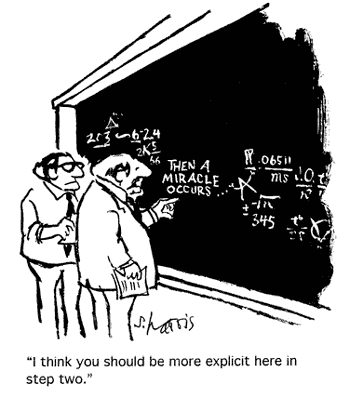
\includegraphics[width=5cm]{math07.png}
  \end{center}
\end{frame}

\begin{frame}{Bibliografía principal}
  \footnotesize
  \begin{thebibliography}{99}

  \bibitem{guinand}
  Guinand, A. P., 
  \textbf{\textit{The umbral method: a survey of elementary mnemonic and manipulative uses}}, 
  Amer. Math. Monthly 86 (1979), no. 3, 187–195.

  \bibitem{bell}
  Bell, E. T., \textbf{\textit{The history of Blissard’s symbolic method, with a sketch of its inventor’s life}}, 
  Amer. Math. Monthly 45 (1938), no. 7, 414–421.

  \bibitem{roman1}
  Roman, Steven, \textbf{\textit{The umbral calculus}}, 
  Pure and Applied Mathematics, 111, Academic Press, Inc., London, 1984.

  \bibitem{kim1}
  Kim, Dae San; Kim, Taekyun, \textbf{\textit{Umbral calculus associated with Bernoulli polynomials}}, J. Number Theory 147 (2015), 871–882.

  \bibitem{costabile}
  Costabile, Francesco, \textbf{\textit{Modern umbral calculus: an elementary introduction with applications to linear interpolation and operator approximation theory}}, De Gruyter, Berlin, (2019).

  \bibitem{kim3}
  T. Kim, D. S. Kim, T. Mansour, S.-H. Rim, and M. Schork, \textbf{\textit{Umbral calculus and Sheffer sequences of polynomials}}, 
  J. Math. Phys. 54 (2013), no. 8, 083504.

  \end{thebibliography}
\end{frame}
  
\end{document}